\part{Literature review}
\frame{\partpage}

\begin{frame}{A typical dissertation structure}
	\begin{itemize}
		\pause\item \textbf{Introduction}: introduce the broad context and motivation,
			culminating in your research question(s)
		\pause\item \textbf{Literature review}: survey existing work related to your project
		\pause\item \textbf{Method}: explain how you went about answering your research question
		\pause\item \textbf{Results}: present and analyse the data obtained, and discuss how it addresses
			your research question
		\pause\item \textbf{Conclusion}: summarise the dissertation, suggest directions for further work
		\pause\item \textbf{References}
	\end{itemize}
\end{frame}

\begin{frame}{The purpose of the literature review}
	\begin{itemize}
		\pause\item Understand the \textbf{context} of your work
		\pause\item Understand the \textbf{state of the art} in the field
			\begin{itemize}
				\pause\item What is currently known?
				\pause\item What are the important open questions?
				\pause\item What research methods are used in the field?
			\end{itemize}
		\pause\item Understand how \textbf{your work} fits in
			\begin{itemize}
				\pause\item Is your work \textbf{novel} (i.e.\ has it not been done before?)
				\pause\item Does it build sensibly on what has come before?
				\pause\item Is your research question one that others have asked, and possibly tried to answer?
			\end{itemize}
	\end{itemize}
\end{frame}

\begin{frame}{Which comes first: research question or literature review?}
	\pause\begin{center}
		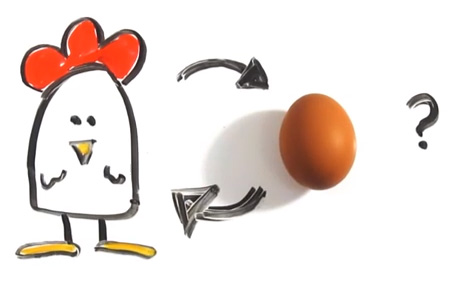
\includegraphics[width=0.4\textwidth]{chickenegg1}
	\end{center}
	\begin{itemize}
		\pause\item Having an initial research question in mind will help focus your literature search
		\pause\item What you read will influence your research question
		\pause\item Be prepared to \textbf{refine} your research question
	\end{itemize}
\end{frame}

\begin{frame}{Tips}
	\begin{itemize}
		\pause\item Read widely!
		\pause\item Keep thorough notes
		\pause\item Annotate (either on paper or on screen)
		\pause\item Write up as you go along
	\end{itemize}
\end{frame}

\begin{frame}{Recommended reading}
	D.\ Boote and P.\ Beile. ``Scholars before researchers: on the centrality of the disseration
		literature review in research preparation,'' \textit{Educational Researcher} Vol.\ 34 No.\ 6, pp.\ 3--15,
		2005.
\end{frame}

\begin{frame}{Examples}
	Some examples of good literature reviews from last year's students are on LearningSpace
\end{frame}
